\documentclass[letterpaper, 11pt]{extarticle}
% \usepackage{fontspec}

% ==================================================

% document parameters
% \usepackage[spanish, mexico, es-lcroman]{babel}
\usepackage[english]{babel}
\usepackage[margin = 1in]{geometry}

% ==================================================

% Packages for math
\usepackage{mathrsfs}
\usepackage{amsfonts}
\usepackage{amsmath}
\usepackage{amsthm}
\usepackage{amssymb}
\usepackage{physics}
\usepackage{dsfont}
\usepackage{esint}

% ==================================================

% Packages for writing
\usepackage{enumerate}
\usepackage[shortlabels]{enumitem}
\usepackage{framed}
\usepackage{csquotes}

% ==================================================

% Miscellaneous packages
\usepackage{float}
\usepackage{tabularx}
\usepackage{xcolor}
\usepackage{multicol}
\usepackage{subcaption}
\usepackage{caption}
\captionsetup{format = hang, margin = 10pt, font = small, labelfont = bf}

% Citation
\usepackage[round, authoryear]{natbib}

% Hyperlinks setup
\usepackage{hyperref}
\definecolor{links}{rgb}{0.36,0.54,0.66}
\hypersetup{
   colorlinks = true,
    linkcolor = black,
     urlcolor = blue,
    citecolor = blue,
    filecolor = blue,
    pdfauthor = {Author},
     pdftitle = {Title},
   pdfsubject = {subject},
  pdfkeywords = {one, two},
  pdfproducer = {LaTeX},
   pdfcreator = {pdfLaTeX},
   }
\usepackage{titlesec}
\usepackage[many]{tcolorbox}

% Adjust spacing after the chapter title
\titlespacing*{\chapter}{0cm}{-2.0cm}{0.50cm}
\titlespacing*{\section}{0cm}{0.50cm}{0.25cm}

% Indent 
\setlength{\parindent}{0pt}
\setlength{\parskip}{1ex}

% --- Theorems, lemma, corollary, postulate, definition ---
% \numberwithin{equation}{section}

\newtcbtheorem[]{problem}{}%
    {enhanced,
    colback = black!5, %white,
    colbacktitle = black!5,
    coltitle = black,
    boxrule = 0pt,
    frame hidden,
    borderline west = {0.5mm}{0.0mm}{black},
    fonttitle = \bfseries,
    breakable,
    before skip = 3ex,
    after skip = 3ex
}{problem}

\tcbuselibrary{skins, breakable}

% --- You can define your own color box. Just copy the previous \newtcbtheorm definition and use the colors of yout liking and the title you want to use.
% --- Basic commands ---
%   Euler's constant
\newcommand{\eu}{\mathrm{e}}

%   Imaginary unit
\newcommand{\im}{\mathrm{i}}

%   Sexagesimal degree symbol
\newcommand{\grado}{\,^{\circ}}

% --- Comandos para álgebra lineal ---
% Matrix transpose
\newcommand{\transpose}[1]{{#1}^{\mathsf{T}}}

%%% Comandos para cálculo
%   Definite integral from -\infty to +\infty
\newcommand{\Int}{\int\limits_{-\infty}^{\infty}}

%   Indefinite integral
\newcommand{\rint}[2]{\int{#1}\dd{#2}}

%  Definite integral
\newcommand{\Rint}[4]{\int\limits_{#1}^{#2}{#3}\dd{#4}}

%   Dot product symbol (use the command \bigcdot)
\makeatletter
\newcommand*\bigcdot{\mathpalette\bigcdot@{.5}}
\newcommand*\bigcdot@[2]{\mathbin{\vcenter{\hbox{\scalebox{#2}{$\m@th#1\bullet$}}}}}
\makeatother

%   Hamiltonian
\newcommand{\Ham}{\hat{\mathcal{H}}}

%   Trace
\renewcommand{\Tr}{\mathrm{Tr}}

% Christoffel symbol of the second kind
\newcommand{\christoffelsecond}[4]{\dfrac{1}{2}g^{#3 #4}(\partial_{#1} g_{#2 #4} + \partial_{#2} g_{#1 #4} - \partial_{#4} g_{#1 #2})}

% Riemann curvature tensor
\newcommand{\riemanncurvature}[5]{\partial_{#3} \Gamma_{#4 #2}^{#1} - \partial_{#4} \Gamma_{#3 #2}^{#1} + \Gamma_{#3 #5}^{#1} \Gamma_{#4 #2}^{#5} - \Gamma_{#4 #5}^{#1} \Gamma_{#3 #2}^{#5}}

% Covariant Riemann curvature tensor
\newcommand{\covariantriemanncurvature}[5]{g_{#1 #5} R^{#5}{}_{#2 #3 #4}}

% Ricci tensor
\newcommand{\riccitensor}[5]{g_{#1 #5} R^{#5}{}_{#2 #3 #4}}

\usepackage{placeins}
\usepackage{listings}
\usepackage{xcolor}

% Define a custom style for VHDL
\lstdefinelanguage{VHDL}{
    keywords=[1]{library, use, entity, is, port, in, out, architecture, of, begin, end, process},
    keywords=[2]{signal, STD_LOGIC, STD_LOGIC_VECTOR},
    keywordstyle=[1]\color{blue}\bfseries,
    keywordstyle=[2]\color{teal}\bfseries,
    sensitive=true,
    morecomment=[l]--,
    morestring=[b]"
}

\lstset{
    language=VHDL,
    basicstyle=\ttfamily\footnotesize,
    numbers=left,
    numberstyle=\tiny\color{gray},
    keywordstyle=\color{blue},
    commentstyle=\color{green!60!black},
    stringstyle=\color{orange},
    breaklines=true,
    showstringspaces=false,
    tabsize=2,
    xleftmargin=2em
}

\begin{document}

\begin{Large}
    \textsf{\textbf{Mini ALU}}\\
\end{Large}
\textbf{Relazione di progetto}

\vspace{1ex}

\textsf{\textbf{Studenti:}} \\
\text{Frega Umberto 239527}, \href{frgmrt04a05l353d@studenti.unical.it}{\texttt{frgmrt04a05l353d@studenti.unical.it}};\\
\text{Napoli Leonardo 234364}, \href{npllrd02s30d086@studenti.unical.it} {\texttt{npllrd02s30d086@studenti.unical.it}};

\href{https://github.com/Zi0LEO/elettronica_digitale}{\texttt{Codice Sorgente}}


\vspace{2ex}

Il progetto assegnato consiste nel progettare ed implementare una mini alu, capace di fare addizioni e sottrazioni, tramite linguaggio VHDL.
Per la progettazione del sistema si è deciso di utilizzare un pattern comportamentale, andando quindi a definire il comportamento del sistema in base a determinate condizioni, oltretutto si è optato per l'utilizzo del tipo \textit{STD\_LOGIC} e quindi \textit{STD\_LOGIC\_VECTOR} per una maggiore flessibilità e maggiori funzionalità.

Il primo passo della progettazione è stato definire la politica tramite la quale la mini ALU potesse cambiare tra addizione e sottrazione. A questo proposito si è deciso di mantenere un singolo adder, ma cambiare
il segno del secondo operando.

\section{Adder}
\subsection{Implementazione}
La componente di base del sistema è un carry look-ahead adder, che genera quindi vari segnali generate e propagate a seconda del numero di bit degli operandi.
Riportiamo di seguito il codice dell'adder con caso di default con 4 bit.

\begin{problem}{Codice adder}{problem-label}
\begin{lstlisting}[language=VHDL]
library IEEE;
use IEEE.STD_LOGIC_1164.ALL;
library work;
use work.constants.all;

entity generic_adder is
    generic (bit_number : INTEGER := nbit);
    Port ( A_adder,B_adder: in STD_LOGIC_VECTOR (bit_number-1 downto 0);
         cin : in STD_LOGIC;
         sum : out STD_LOGIC_VECTOR (bit_number downto 0));
end generic_adder;

architecture Behavioral of generic_adder is
    signal p,g : STD_LOGIC_VECTOR (bit_number downto 0);
    signal carry : STD_LOGIC_VECTOR (bit_number+1 downto 0);
begin
    carry(0) <= cin;
    p_g: for i in 0 to bit_number generate
        p_gMSB: if (i=bit_number) generate
            p(i) <= A_adder(bit_number-1) xor B_adder(bit_number-1);
            g(i) <= A_adder(bit_number-1) and B_adder(bit_number-1);
        end generate;
        p_gLSB: if i<bit_number generate
            p(i) <= A_adder(i) xor B_adder(i);
            g(i) <= A_adder(i) and B_adder(i);
        end generate;
        carry(i+1) <= (g(i) or (p(i) and carry(i)));
        sum(i) <= carry(i) xor p(i);
    end generate;
end Behavioral;
\end{lstlisting}
\end{problem}

\subsection{Schematica}
Il codice precedente con bit number 4, 8 e 16 ha generato in vivado le schematiche riportate rispettivamente in \textit{Figure 1}, \textit{Figure 2}, \textit{Figure 3}.

\begin{figure}[ht]
    \centering
    \begin{minipage}{0.45\textwidth}
    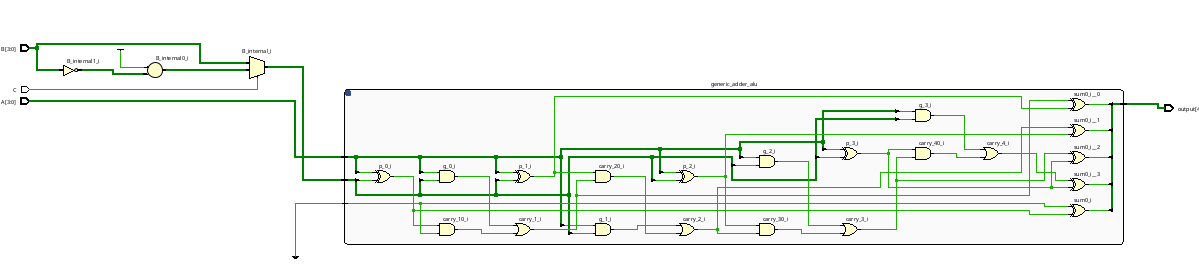
\includegraphics[width=1\textwidth]{assets/schematics/generic_4bit.png}
    \caption{Adder a 4 bit}
  \end{minipage}
    \begin{minipage}{0.45\textwidth}
    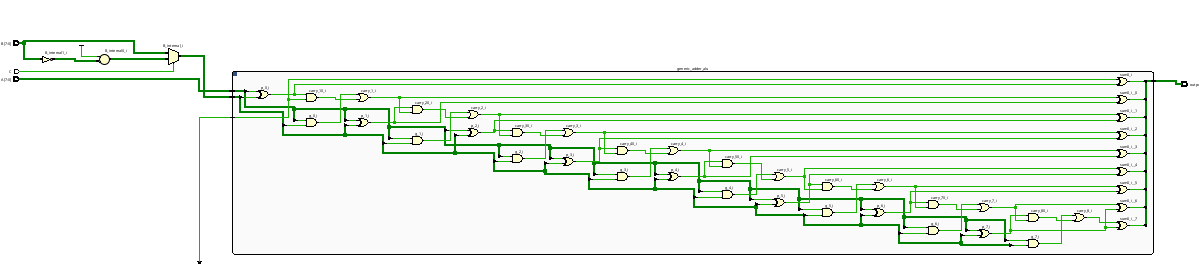
\includegraphics[width=1\textwidth]{assets/schematics/generic_8bit.png}
    \caption{Adder a 8 bit}
  \end{minipage}
    \begin{minipage}{1\textwidth}
    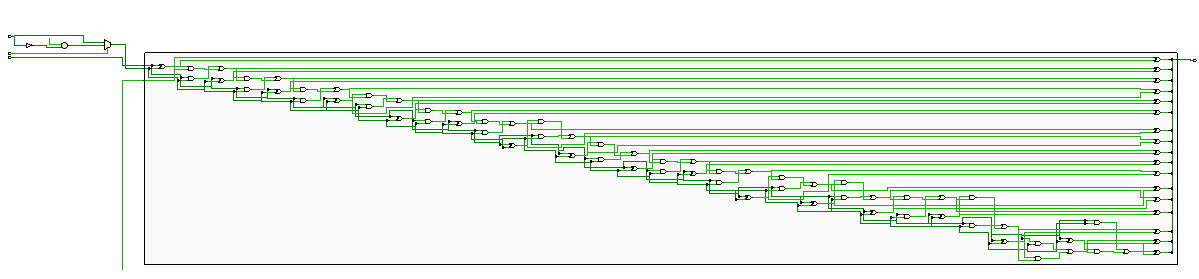
\includegraphics[width=1\textwidth]{assets/schematics/generic_16bit.png}
    \caption{Adder a 16 bit}
  \end{minipage}
\end{figure}
\clearpage

\section{Mini ALU}
\subsection{Implementazione}
La mini ALU progettata presenta al suo interno un solo adder, preceduto da un multiplexer, che in base al bit di controllo C decide se dare in output B oppure il risultato di B invertito.
Nell'adder poi, oltre ad A ed al valore calcolato di B, verrà introdotto il valore di C stesso, completando il complemento a 2 in caso di necessità, non apportando cambiamenti altrimenti.

\begin{problem}{Codice Mini ALU}{}
\begin{lstlisting}[language=VHDL]
library IEEE;
use IEEE.STD_LOGIC_1164.ALL;
library work;
use work.constants.all;

entity mini_alu is
  generic (bit_number : INTEGER := nbit);
    Port ( A,B : in STD_LOGIC_VECTOR (bit_number-1 downto 0);
           C : in STD_LOGIC;
           output : out STD_LOGIC_VECTOR (bit_number downto 0));
end mini_alu;

architecture Behavioral of mini_alu is
  component generic_adder is
    generic (bit_number:INTEGER := nbit);
      Port ( 
        A_adder, B_adder : in STD_LOGIC_VECTOR (bit_number-1 downto 0);
        cin : in STD_LOGIC;
       sum : out STD_LOGIC_VECTOR (bit_number downto 0));
  end component;

signal B_internal: STD_LOGIC_VECTOR (bit_number-1 downto 0);
signal carry_in: STD_LOGIC;

begin
  process(A, B, C) begin
    case C is
      when '0' => 
      B_internal <= B;
            
      when others =>
      B_internal <= STD_LOGIC_VECTOR(not B);

    end case;
  end process;

generic_adder_alu: generic_adder 
      GENERIC MAP (bit_number => bit_number)
      PORT MAP (
      A_adder => A,
      B_adder => B_internal,
      cin => C,
      sum => output);
end Behavioral
\end{lstlisting}
\end{problem}

Possiamo trovare la schematica risultante nella \textit{Figure 4}
\begin{figure}[ht]
    \centering
    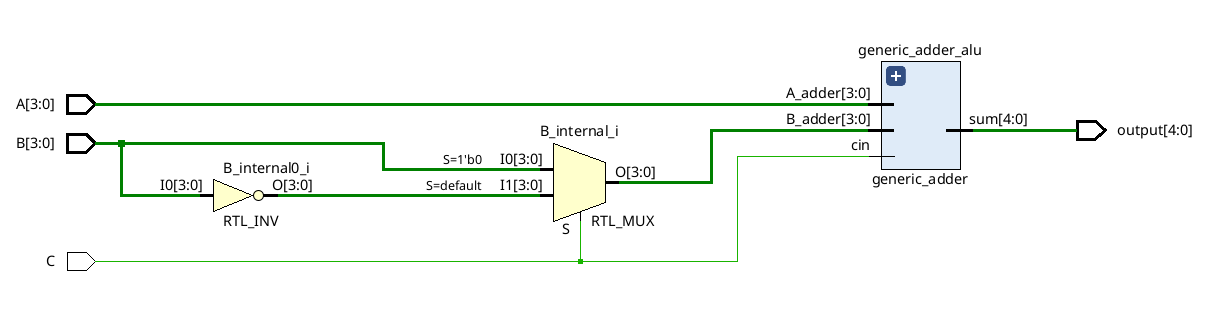
\includegraphics[width=15cm]{assets/schematics/generic_alu.png}
    \caption{Circuito Logico del mini ALU}
\end{figure}

\subsection{TestBench}
I test sono stati svolti in tutti i casi possibili, dando un tempo di 10 ns per ogni caso, con un tempo totale in nanosecondi: \begin{equation}2^{2n+1} \times 10\end{equation}

\begin{problem}{Codice test}{}
\begin{lstlisting}[language=VHDL]
library IEEE;
use IEEE.STD_LOGIC_1164.ALL;
use IEEE.NUMERIC_STD.all;
library work;
use work.constants.all;

entity mini_alu_testbench is
    generic (bit_number: integer := nbit);
end mini_alu_testbench;

architecture Behavioral of mini_alu_testbench is
    component mini_alu is
    generic (bit_number : INTEGER := nbit);
    Port ( A,B : in STD_LOGIC_VECTOR (bit_number-1 downto 0);
           C : in STD_LOGIC;
           output : out STD_LOGIC_VECTOR (bit_number downto 0));
    end component;
    
    constant min_value : integer := -(2**(bit_number-1));
    constant max_value : integer := (2**(bit_number-1))-1;

    signal Ia,Ib: STD_LOGIC_VECTOR (bit_number-1 downto 0);
    signal Ic: STD_LOGIC;
    signal Ooutput: STD_LOGIC_VECTOR(bit_number downto 0);
begin 
    CUT: mini_alu port map(Ia,Ib,Ic, Ooutput);
    process 
    begin
      external: for i in min_value to max_value loop
          Ia <= (STD_LOGIC_VECTOR((TO_SIGNED(i,bit_number))));
          internal: for j in min_value to max_value loop
            Ic <= '0';
            Ib <= (STD_LOGIC_VECTOR((TO_SIGNED(j,bit_number))));
            wait for 10ns;
            Ic <= '1';
            wait for 10ns;
         end loop internal;
       end loop external;   
    end process;
end Behavioral;
\end{lstlisting}
\end{problem}

\clearpage
\section{Simulazione}
Sono state effettuate simulazioni behavioural e post-implementation. Vediamole, evidenziandone le differenze.

\subsection{4 bit}
Per prime analizziamo le simulazioni nel caso del circuito a 4 bit.
Per semplicita verranno riportate solo le immagini di alcuni momenti salienti della simulazione
\subsubsection{Behavioural}
\begin{figure}[ht]
      \centering
      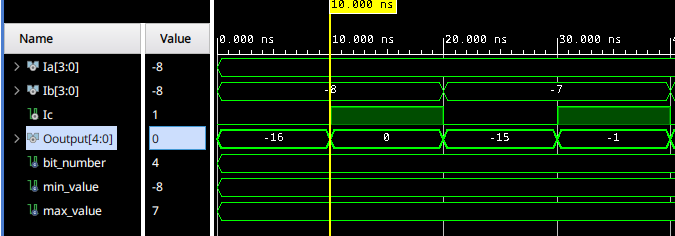
\includegraphics[width=1\textwidth]{assets/simulations/behavioural/4bit/4bit_behav.png}
      \caption{Cambio di Ic}
      \label{4bit_behav}
\end{figure}

Possiamo notare come la simulazione in \textit{Figure~\ref{4bit_behav}} restituisca i dati corretti senza nessun delay. Vediamo ora la stessa situazione in
un'implementazione reale.

\subsubsection{Post-implementation}
\begin{figure}[ht]
      \centering
      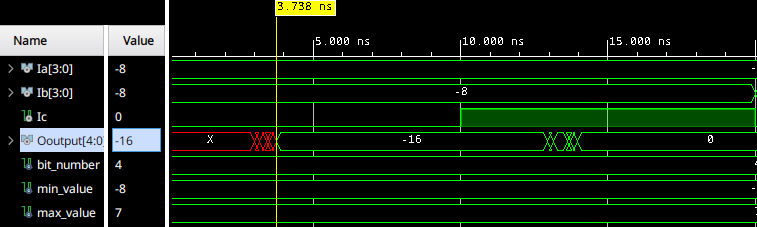
\includegraphics[width=1\textwidth]{assets/simulations/Post_Implementation/4bit/end_X.png}
      \caption{Fine output non definito}
      \label{4bit_pi_x}
\end{figure}

Degna di nota la prima differenza mostrata in \textit{Figure~\ref{4bit_pi_x}}, nonostante gli input vengano dati al tempo iniziale 0, sono necessari 3,738 ns affinche 
il circuito produca il primo risultato utile.

\begin{figure}[ht]
      \centering
      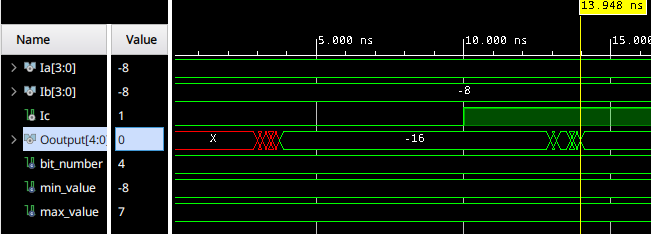
\includegraphics[width=1\textwidth]{assets/simulations/Post_Implementation/4bit/C_change.png}
      \caption{Cambio di C}
      \label{4bit_pi_c}
\end{figure}

Ancora, affinchè il risultato del cambio di valore di C possa essere utilizzato sono necessari 3,948 ns, come si vede in \textit{Figure~\ref{4bit_pi_c}}

\begin{figure}[ht]
      \centering
      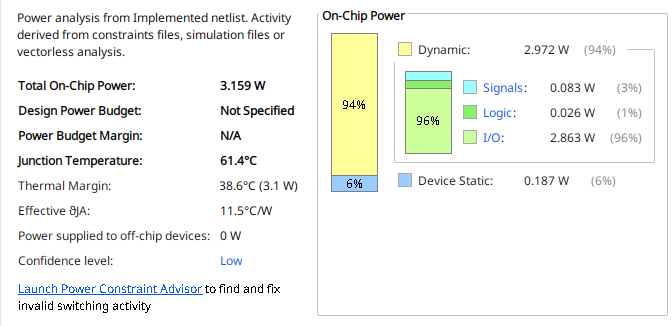
\includegraphics[width=1\textwidth]{assets/simulations/Post_Implementation/4bit/power.png}
      \caption{Junction Temperature e Total Power}
      \label{4bit_power}
\end{figure}

Da \textit{Figure~\ref{4bit_power}} notiamo che l'implementazione del circuito, sebbene non presenti un clock, non produce problemi significativi dal punto di vista della temperatura, grazie al basso numero di bit da calcolare.
\FloatBarrier

\subsubsection{LUT Tables}

Dalla sintesi del circuito ci vengono restituite inoltre le LUT Tables con i relativi valori di utilizzo. Il loro numero è riportato in \textit{Table~\ref{lut_quantity_4bit}}, mentre in \textit{Figure~\ref{lut_schematic_4bit}}
troviamo la schematica del circuito reale.

\begin{table}[ht]
      \centering
      \begin{tabular}{|c|c|c|}
        \hline
        Nome & Utilizzate & Tipo di utilizzo \\ \hline
        IBUF & 9 & IO \\ \hline
        OBUF & 5 & IO \\ \hline
        LUT6 & 2 & LUT \\ \hline
        LUT5 & 2 & LUT \\ \hline
        LUT4 & 1 & LUT \\ \hline
        LUT2 & 1 & LUT \\ \hline 
      \end{tabular}
      \caption{Numero LUT utilizzati nel circuito a 4 bit}
      \label{lut_quantity_4bit}
\end{table}
\begin{figure}[ht]
  \centering
  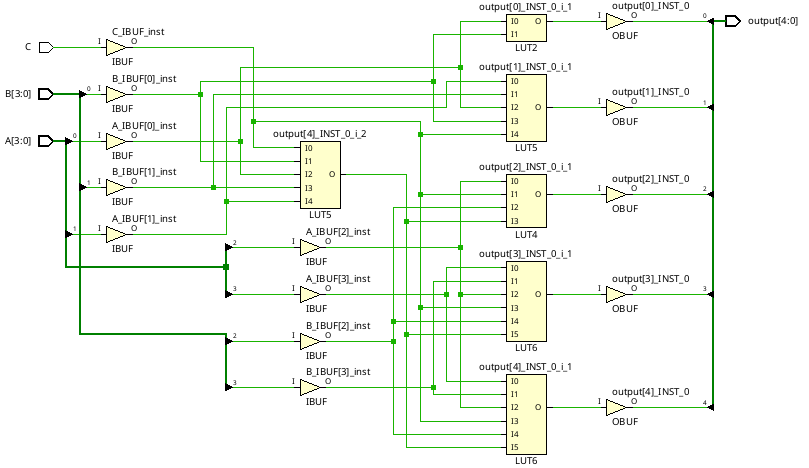
\includegraphics[width=1\textwidth]{assets/LUT/4bit/LUT_schematic_4bit.png}
  \caption{Schematica circuito reale}
  \label{lut_schematic_4bit} 
\end{figure}

Riportiamo per completezza in \textit{Table~\ref{lut_utilization_4bit}} anche l'utilizzazione delle LUT, estremamente bassa a causa della semplicità del circuito
\begin{table}[ht]
      \centering
      \begin{tabular}{|c|c|c|c|c|c|}
        \hline
        Site Type & Used & Fixed & Prohibited & Available & Util\% \\ \hline
        Slice LUTs & 5 & 0 & 0 & 53200 & $<0.01$ \\ \hline
         LUT as Logic & 5 & 0 & 0 & 53200 & $<0.01$ \\ \hline 
         LUT as Memory  & 0 & 0 & 0 & 17400 & $0.00$ \\ \hline
      \end{tabular}
      \caption{Numero LUT utilizzati nel circuito a 4 bit}
      \label{lut_utilization_4bit}
\end{table}
\FloatBarrier

\subsection{8 bit}
Analizziamo ora le simulazioni ottenute nel caso di circuito a 8 bit. 
\subsubsection{Behavioural}
La \textit{Figure~\ref{8bit_behav}} illustra la simulazione behavioural, quindi ideale.

\begin{figure}[ht]
  \centering
  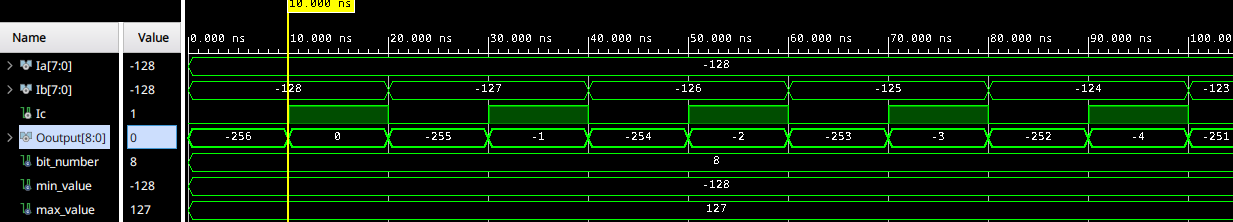
\includegraphics[width=1\textwidth]{assets/simulations/behavioural/8bit/8bit_behav_sim.png}
  \caption{Simulazione 8 bit}
  \label{8bit_behav} 
\end{figure}

\subsubsection{Post-implementation}
Passando alla simulazione post-implementation, notiamo che il ritardo inizia a diventare piuttosto importante. Dalla \textit{Figure~\ref{8bit_pi_x}} vediamo infatti che per avere il primo valore utile saranno necessari 
ben 7,5 ns sui 10 totali concessi.
\begin{figure}[ht]
  \centering
  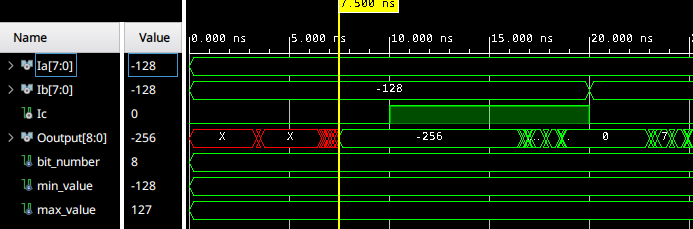
\includegraphics[width=1\textwidth]{assets/simulations/Post_Implementation/8bit/end_x.png}
  \caption{Primo valore utile}
  \label{8bit_pi_x} 
\end{figure}

Negli istanti successivi il valore del ritardo tende ad assestarsi su una media di circa 7 ns dalla ricezione degli input all'invio dell'output corretto, come visibile dall'esempio generico della \textit{Figure~\ref{random_val}}
\begin{figure}[ht]
  \centering
  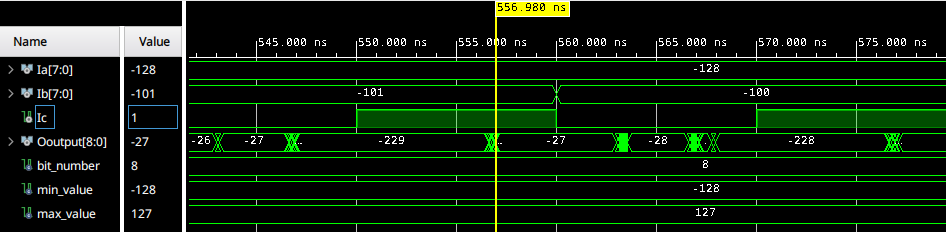
\includegraphics[width=1\textwidth]{assets/simulations/Post_Implementation/8bit/random_val.png}
  \caption{Dimostrazione ritardo di 6,98 ns}
  \label{random_val} 
\end{figure}

Dal punto di vista della temperatura il circuito ad 8 bit inizia a risentire della mancanza di un clock. La \textit{Figure~\ref{8bit_power}} infatti mostra una temperatura massima raggiunta di oltre
100 gradi, che rischia di compromettere la stabilità ed il funzionamento di un circuito reale.
\begin{figure}[ht]
  \centering
  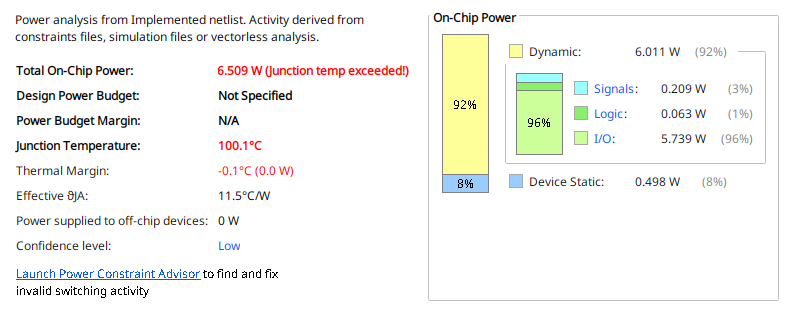
\includegraphics[width=1\textwidth]{assets/simulations/Post_Implementation/8bit/power.png}
  \caption{Total On-Chip Power e Junction Temperature}
  \label{8bit_power} 
\end{figure}
\FloatBarrier

\subsubsection{LUT Tables}
Le tables utilizzate nel circuito a 8 bit sono maggiori di quelle del circuito a 4 bit, come vediamo dalle quantità mostrate in \textit{Table~\ref{lut_quantity_8bit}} e dalla loro disposizione,
evidenziata in \textit{Figure~\ref{lut_schematic_8bit}}
\begin{table}[ht]
      \centering
      \begin{tabular}{|c|c|c|}
        \hline
        Nome & Utilizzate & Tipo di utilizzo \\ \hline
        IBUF & 17 & IO \\ \hline
        OBUF & 9 & IO \\ \hline
        LUT6 & 6 & LUT \\ \hline
        LUT5 & 3 & LUT \\ \hline
        LUT4 & 2 & LUT \\ \hline
        LUT2 & 1 & LUT \\ \hline 
      \end{tabular}
      \caption{Numero LUT utilizzati nel circuito a 8 bit}
      \label{lut_quantity_8bit}
\end{table}
\begin{figure}[ht]
  \centering
  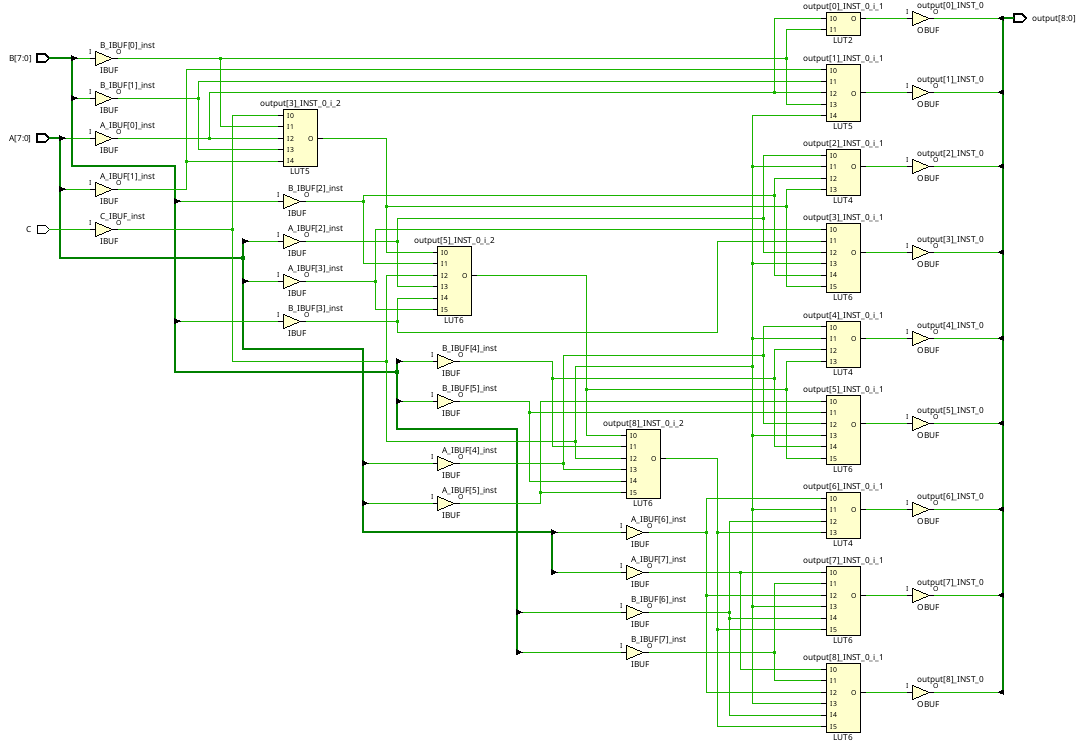
\includegraphics[width=1\textwidth]{assets/LUT/8bit/LUT_schematic_8bit.png}
  \caption{Schematica circuito reale}
  \label{lut_schematic_8bit}
\end{figure}

Nonostante questi incrementi, l'utilizzazione mostrata in figura \textit{Table~\ref{lut_utilization_8bit}} rimane minima.

\begin{table}[ht]
      \centering
      \begin{tabular}{|c|c|c|c|c|c|}
        \hline
        Site Type & Used & Fixed & Prohibited & Available & Util\% \\ \hline
        Slice LUTs & 11 & 0 & 0 & 53200 & $0.02$ \\ \hline
         LUT as Logic & 11 & 0 & 0 & 53200 & $0.02$ \\ \hline 
         LUT as Memory  & 0 & 0 & 0 & 17400 & $0.00$ \\ \hline
      \end{tabular}
      \caption{Numero LUT utilizzati nel circuito a 4 bit}
      \label{lut_utilization_8bit}
\end{table}

\clearpage
\subsection{16 Bit}
Per la sezione finale andremo ad analizzare il comportamento della nostra mini alu inl caso in cui abbia 16 bit.

\subsubsection{Behavioural}
Riportiamo nella \textit{Figure~\ref{16bit_behav}} simulazione behavioural, per avere un modello di riferimento.
\begin{figure}[ht]
  \centering
  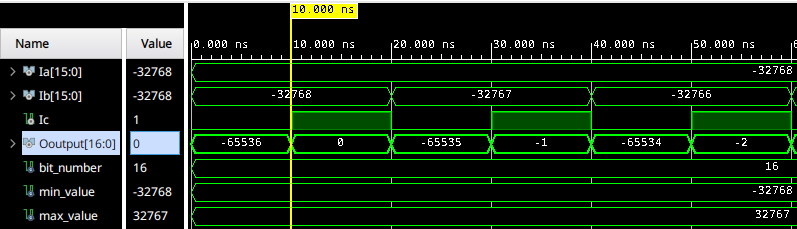
\includegraphics[width=1\textwidth]{assets/simulations/behavioural/16bit/16bit_behav.png}
  \caption{Simulazione ideale a 16 bit}
  \label{16bit_behav}
\end{figure}
\FloatBarrier

\subsubsection{Post-implementation}
Analizziamo adesso la simulazione post-implementation, ponendo ancora una volta la lente d'ingrandimento sui ritardi temporali rapportati alla simulazione ideale.
Dalla \textit{Figure~\ref{16bit_pi_x}} risulta evidente che questa implementazione presenta dei problemi non indifferenti. A fronte dell'input iniziale dei classici 10 ns, ne saranno necessari 11,817 per
produrre il primo risultato utile, portando ad uno sfasamento per cui il risultato di un input verrà mostrato soltanto quando l'input successivo sarà già stato ricevuto
\begin{figure}[ht]
  \centering
  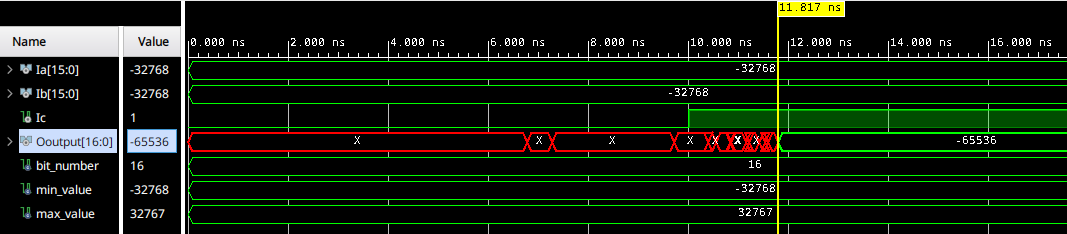
\includegraphics[width=1\textwidth]{assets/simulations/Post_Implementation/16bit/end_x.png}
  \caption{Primo valore utile}
  \label{16bit_pi_x} 
\end{figure}

Prendendo un istante di tempo generico, nel nostro caso fissato a 11,911,821.768 ns, avremo come output -5757, risultato degli input somministrati all'istante 11,911,810.000 ns, \textit{Figure~\ref{random_val16}}.
Da questo e da altri casi campionati possiamo affermare che il ritardo medio che si verifica consiste proprio nel valore iniziale osservato di 11,8 ns.
\begin{figure}[ht]
  \centering
  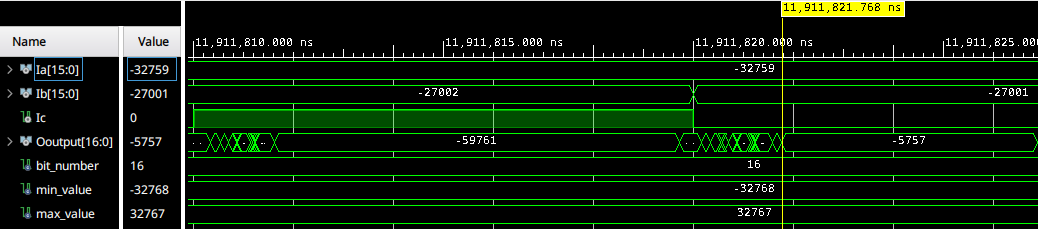
\includegraphics[width=1\textwidth]{assets/simulations/Post_Implementation/16bit/random_val.png}
  \caption{Dimostrazione ritardo di 11,8 ns}
  \label{random_val16} 
\end{figure}

La temperatura del circuito raggiunge una quota insostenibile, a fronte di una potenza di 14,276 w. La temperatura di giunzione mostrata in \textit{Figure~\ref{16bit_power}} non può considerarsi 
accurata in quanto Vivado la possiede un limite massimo a 125 gradi Celsius, che verrebbero quindi ampiamente superati.
\begin{figure}[ht]
  \centering
  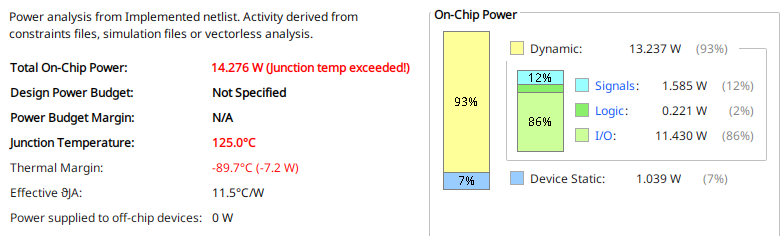
\includegraphics[width=1\textwidth]{assets/simulations/Post_Implementation/16bit/power.png}
  \caption{Total On-Chip Power e Junction Temperature}
  \label{16bit_power} 
\end{figure}
\FloatBarrier

\subsubsection{LUT Tables}
Le tables utilizzate nel circuito continuano ad aumentare con l'aumentare del numero di bit, come dimostra la \textit{Table~\ref{lut_quantity_16bit}}. Riportiamo anche la schematica reale in \textit{Figure~\ref{lut_schematic_16bit}}
\begin{table}[ht]
      \centering
      \begin{tabular}{|c|c|c|}
        \hline
        Nome & Utilizzate & Tipo di utilizzo \\ \hline
        IBUF & 33 & IO \\ \hline
        LUT6 & 21 & LUT \\ \hline
        OBUF & 17 & IO \\ \hline
        LUT5 & 9 & LUT \\ \hline
        LUT4 & 4 & LUT \\ \hline
        LUT2 & 2 & LUT \\ \hline 
      \end{tabular}
      \caption{Numero LUT utilizzati nel circuito a 16 bit}
      \label{lut_quantity_16bit}
\end{table}
\begin{figure}[ht]
  \centering
  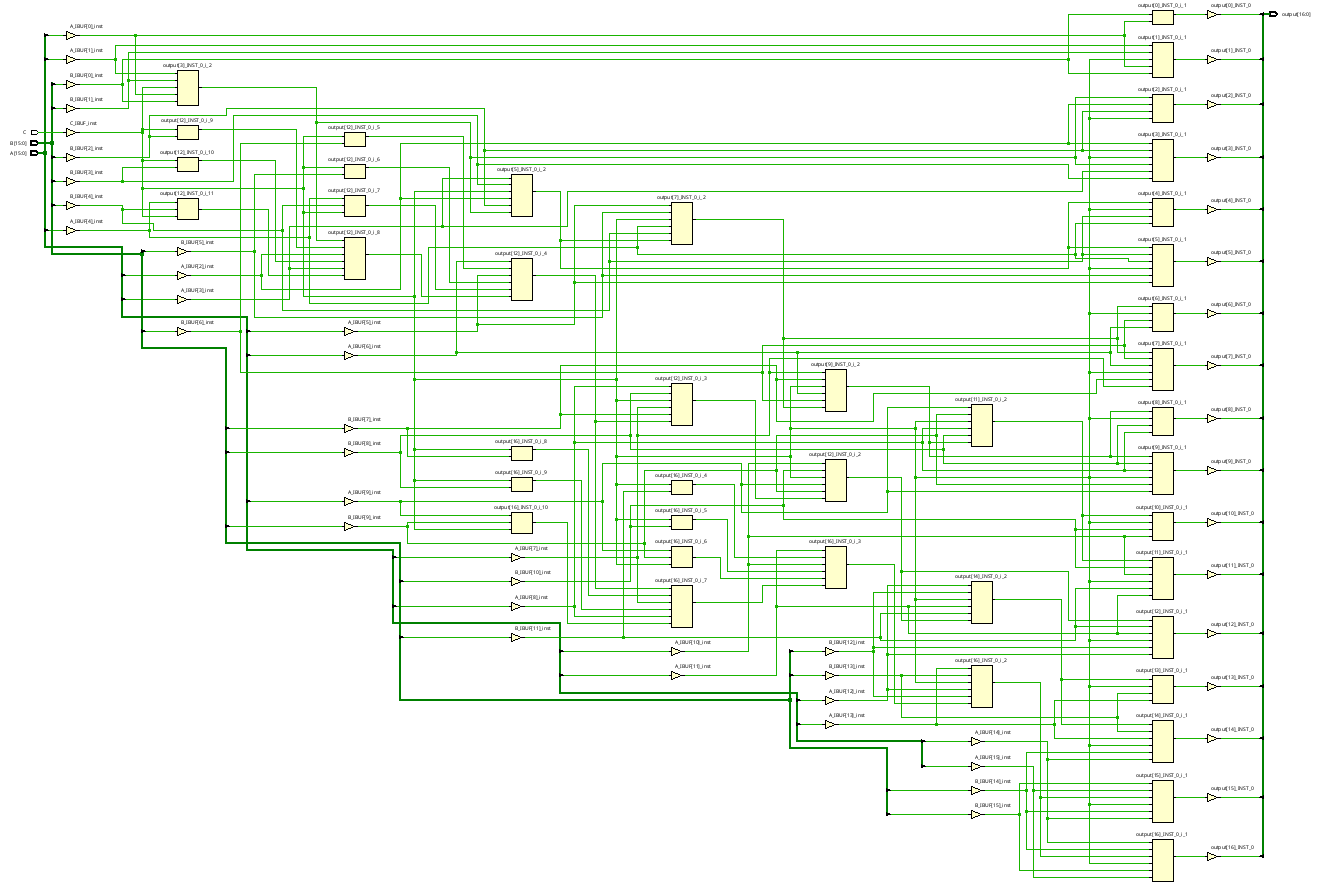
\includegraphics[width=1\textwidth]{assets/LUT/16bit/LUT_schematic_16bit.png}
  \caption{Schematica circuito reale}
  \label{lut_schematic_16bit}
\end{figure}

L'utilizzazione è invece riportata in \textit{Table~\ref{lut_utilization_16bit}}
\begin{table}[ht]
      \centering
      \begin{tabular}{|c|c|c|c|c|c|}
        \hline
        Site Type & Used & Fixed & Prohibited & Available & Util\% \\ \hline
        Slice LUTs & 32 & 0 & 0 & 53200 & $0.06$ \\ \hline
         LUT as Logic & 32 & 0 & 0 & 53200 & $0.06$ \\ \hline 
         LUT as Memory  & 0 & 0 & 0 & 17400 & $0.00$ \\ \hline
      \end{tabular}
      \caption{Numero LUT utilizzati nel circuito a 4 bit}
      \label{lut_utilization_16bit}
\end{table}

\end{document}
